% Präambel
\documentclass[
fontsize=12pt,
paper=a4,						
twoside=false, 					
listof=totoc, 					
bibliography=totoc,				
titlepage, 					
%headsepline, 					% horizontale Linie unter Kolumnentitel
%abstracton,					% Überschrift beim Abstract einschalten, Abstract muss dazu in {abstract}-Umgebung stehen
DIV=12,						
%BCOR=6mm,						% Bindekorrektur, die den Seitenspiegel um 6mm nach rechts verschiebt,
cleardoublepage=empty,			
parskip,				
ngerman
]{scrbook}
\usepackage[left=2.5cm, 
			right=2.5cm,
			top=2.5cm, 
			bottom=3.2cm, 
			headsep=1cm, 
			footskip=1.6cm]{geometry}
\usepackage{times}		
\usepackage[setspace=false]{scrhack}
\usepackage[utf8]{inputenc} 	
\usepackage[T1]{fontenc} 		
\usepackage{babel} 			
\setlength{\parindent}{0ex} 	
\usepackage[onehalfspacing]{setspace}

%------

\usepackage{siunitx}			
\sisetup{
	number-unit-product = \;,
	inter-unit-product = \:,
	exponent-product = \cdot,
	output-decimal-marker = {,}
}

\usepackage{graphicx}  			
\usepackage[format=hang,		
font=normal,
labelfont=bf,
justification=RaggedRight,
singlelinecheck=true,
aboveskip=1mm
]{caption}

\usepackage[backend=biber, 		
style=numeric, 				
natbib=true, 					
hyperref=true, 					
]{biblatex}
\setcounter{biburllcpenalty}{7000}
\setcounter{biburlucpenalty}{8000}
\addbibresource{literature/literatur1.bib} %% Einbinden der bib-Datei. Endung .bib unbedingt ergänzen
\addbibresource{literature/literatur2.bib} %% Einbinden mehrerer bib-Dateien mit zusätzlichem \addbibresource - Befehl

\usepackage{csquotes}

% Folgende Zeilen sind auszukommentieren, falls runde Klammern und ein vgl. bei Zitaten erscheinen sollen.
%\makeatletter
%\renewcommand{\@cite}[2]{(vgl. {#1\if@tempswa , #2\fi})} 
%\renewcommand{\@biblabel}[1]{(#1)}
%\makeatother

\usepackage{pdfpages}

\usepackage{enumitem}			
\usepackage{amsmath}	
\usepackage{mhchem}		
\usepackage{textcomp} 			
\usepackage{eurosym}			% Bessere Darstellung Euro-Symbol mit \euro

\usepackage[					
hyperfootnotes=false,			
hidelinks						
]{hyperref}

\usepackage{acronym}

\usepackage{makeidx}			% Paket zur Erstellung eines Index
\usepackage[intoc]{nomencl} 	% zur Erstellung des Abkürzungsberzeichnisses

\usepackage[					% Einstellungen für Fußnoten
bottom,							% Ausrichtung unten
multiple,						% Trennung durch Seperator bei mehreren Fußnoten
hang,
marginal
]{footmisc}

\usepackage{calc}				% Paket zum Berechnen von Längen z.B. 0.8\linewidth

\usepackage{xcolor} 			% einfache Verwendung von Farben in nahezu allen Farbmodellen

\usepackage{listings}			% Darstellung von Quellcode mit den Umgebungen {lstlisting}, \lstinline und \lstinputlisting
\lstset{literate=				% Damit können Umlaute innerhalb Listings geschrieben werden
	{Ö}{{\"O}}1
	{Ä}{{\"A}}1
	{Ü}{{\"U}}1
	{ß}{{\ss}}1
	{ü}{{\"u}}1
	{ä}{{\"a}}1
	{ö}{{\"o}}1
}
\definecolor{mygreen}{rgb}{0,0.6,0}
\definecolor{mygray}{rgb}{0.5,0.5,0.5}
\definecolor{mymauve}{rgb}{0.58,0,0.82}
\lstset{ %
	backgroundcolor=\color{white},   % choose the background color; you must add \usepackage{color} or \usepackage{xcolor}; should come as last argument
	basicstyle=\footnotesize,        % the size of the fonts that are used for the code
	breakatwhitespace=false,         % sets if automatic breaks should only happen at whitespace
	breaklines=true,                 % sets automatic line breaking
	captionpos=t,                    % sets the caption-position to (b) bottom or (t) top
	commentstyle=\color{mygreen},    % comment style
	deletekeywords={...},            % if you want to delete keywords from the given language
	escapeinside={\%*}{*)},          % if you want to add LaTeX within your code
	escapeinside={(*@}{@*)},
	extendedchars=true,              % lets you use non-ASCII characters; for 8-bits encodings only, does not work with UTF-8
	frame=none,	                   	 % "single" adds a frame around the code; "none"
	keepspaces=true,                 % keeps spaces in text, useful for keeping indentation of code (possibly needs columns=flexible)
	keywordstyle=\color{blue},       % keyword style
	language=[LaTeX]TeX,             % the language of the code
	morekeywords={*,nomenclature},   % if you want to add more keywords to the set
	numbers=left,                    % where to put the line-numbers; possible values are (none, left, right)
	numbersep=5pt,                   % how far the line-numbers are from the code
	numberstyle=\tiny\color{mygray}, % the style that is used for the line-numbers
	rulecolor=\color{black},         % if not set, the frame-color may be changed on line-breaks within not-black text (e.g. comments (green here))
	showspaces=false,                % show spaces everywhere adding particular underscores; it overrides 'showstringspaces'
	showstringspaces=false,          % underline spaces within strings only
	showtabs=false,                  % show tabs within strings adding particular underscores
	stepnumber=1,                    % the step between two line-numbers. If it's 1, each line will be numbered
	stringstyle=\color{mymauve},     % string literal style
	tabsize=2,	                   % sets default tabsize to 2 spaces
	title=\lstname                   % show the filename of files included with \lstinputlisting; also try caption instead of title
}

\makeindex						% Indexverzeichnis erstellen
\makenomenclature				% Abkürzungsverzeichnis erstellen

% -----------------------------------------------------------------------------------------------------------------
% Zum Aktualisieren des Abkürzungsverzeichnisses (Nomenklatur) bitte auf der Kommandozeile folgenden Befehl aufrufen :
% makeindex <Dateiname>.nlo -s nomencl.ist -o <Dateiname>.nls
% Oder besser: Kann in TexStudio unter Tools-Benutzer als Shortlink angelegt werden
% Konfiguration unter: Optionen-Erzeugen-Benutzerbefehle: makeindex -s nomencl.ist -t %.nlg -o %.nls %.nlo
% -----------------------------------------------------------------------------------------------------------------

% Hier die persönlichen Daten eingeben:

\newcommand{\titel}{Grundlagen der Metallbearbeitung und Einführung in den Betrieb des Stromnetzes der TWS Netz GmbH}
%\newcommand{\untertitel}{}			% ggf. Untertitel mit ergänzenden Hinweisen
\newcommand{\arbeit}{Praxisarbeit T3\_1000}
\newcommand{\studiengang}{Elektrotechnik}
\newcommand{\studienrichtung}{Energie- und Umwelttechnik}
\newcommand{\studienschwerpunkt}{}
\newcommand{\autor}{Alexander Dreher}
\newcommand{\matrikelnr}{5642939}
\newcommand{\kurs}{TFE22-1/TEU22}
\newcommand{\firma}{TWS Netz GmbH}
\newcommand{\abgabe}{\today}
\newcommand{\betreuerdhbw}{}			% Gutachter der DHBW (nur bei Bachelorarbeit erforderlich)
\newcommand{\betreuerfirma}{Patricia Schmitz}
\newcommand{\jahr}{2023}			% für Angabe im Copyright-Vermerk der Titelseite

% Folgende Zeilen definieren Abkürzungen, um Befehle schneller eingeben zu können
\newcommand{\ua}{\mbox{u.\,a.\ }}
\newcommand{\zB}{\mbox{z.\,B.\ }}
\newcommand{\bs}{$\backslash$}
\newcommand*\diff{\mathop{}\!\mathrm{d}}	% Differentialzeichen
\newcommand*\Diff[1]{\mathop{}\!\mathrm{d^#1}} % Differentialzeichen höherer Ableitung
\newcommand*\jj{\mathop{}\!\mathrm{j}}	% Komplexe Zahl j

% Folgende Zeilen werden benötigt, um Tikz und PGF-Plot-Grafiken einzubinden
\usepackage{pgfplots}
\usepackage{pgfplotstable}
\pgfplotsset{compat=newest,width=0.6\linewidth}
\usepgfplotslibrary{smithchart}
\usepackage{tikz}						% Tikz sollte nach Listings Pakete geladen werden.
\usetikzlibrary{arrows}

\hyphenation{Schrift-ar-ten}


% -------------------------------------------------------------------------------------------
%                     Beginn des Dokumenteninhalts
% -------------------------------------------------------------------------------------------
\begin{document}
\let\texteuro\euro						% Eingabe \texteuro, € oder \euro erzeugt gleiches Ergebnis
\setcounter{secnumdepth}{3}				% Nummerierungstiefe fürs Inhaltsverzeichnis
\setcounter{tocdepth}{3}
\sffamily								% für die Titelei serifenlose Schrift verwenden

% ------------------------------ Titelei -----------------------------------------------------

\thispagestyle{plain}
\hypersetup{pageanchor=false}
\begin{titlepage}
\enlargethispage{4.0cm}
\sffamily 								% Serifenlose Grundschrift für die Titelseite einstellen

\parbox{0.5\linewidth}{
\begin{flushleft}
	\includegraphics[width=0.5\linewidth]{images/Firmenlogo}\\[5ex]
\end{flushleft}
}
\parbox{0.5\linewidth}{
\begin{flushright}
	
\includegraphics[width=0.5\linewidth]{images/DHBW_d_R_FN_46mm_4c}\\[5ex]
\end{flushright}
}
				

\begin{center}

{\fontsize{20.74pt}{24pt}\selectfont
\textbf{\titel}\\[1.5ex]}
{\fontsize{14pt}{17pt}\selectfont
\textbf{\untertitel}\\[5ex]}
{\fontsize{17pt}{20pt}\selectfont
\textbf{\arbeit}\\[2ex]}
{\fontsize{14pt}{17pt}\selectfont
Studiengang \studiengang\\[2ex]}
{\fontsize{12pt}{14pt}\selectfont
Studienrichtung \studienrichtung\\[1ex]
Duale Hochschule Baden-Württemberg Ravensburg, Campus Friedrichshafen\\[5ex]
von\\[1ex]
\autor\\[15ex]}


\end{center}

\begin{flushleft}
{\fontsize{12pt}{14pt}\selectfont
\begin{tabular}{ll}
Abgabedatum:					& \quad \abgabe \\
Bearbeitungszeitraum:		   		& \quad 01.07.2023 - 31.09.2023   \\ 
Matrikelnummer: 			& \quad \matrikelnr \\ 
Kurs: 							& \quad \kurs \\
Ausbildungsfirma:	 			& \quad \firma \\ 
Betreuer der Ausbildungsfirma:  & \quad \betreuerfirma \\ 
%Gutachter der Dualen Hochschule: & \quad \betreuerdhbw \\ [2ex]
\end{tabular}
}
\end{flushleft}
%%%%% Nachfolgende Zeilen einkommentieren, wenn Copyrightvermerk gewünscht ist
%\begin{flushleft}
%{\fontsize{11pt}{13pt}\selectfont
%Copyrightvermerk:\\
%Dieses Werk einschließlich seiner Teile ist \textbf{urheberrechtlich geschützt}. Jede Verwertung außerhalb der engen Grenzen des Urheberrechtgesetzes ist ohne Zustimmung des Autors unzulässig und strafbar. Das gilt insbesondere für Vervielfältigungen, Übersetzungen, Mikroverfilmungen sowie die Einspeicherung und Verarbeitung in elektronischen Systemen.
%}
%\end{flushleft}
%\begin{flushright}
%{\fontsize{11pt}{13pt}\selectfont \copyright{} \jahr }
%\end{flushright}
\end{titlepage}

\cleardoublepage
\hypersetup{pageanchor=true}
 				% erzeugt die Titelseite
\pagenumbering{roman}					% kleine, römische Seitenzahlen für Titelei
%% Ggf. folgende Zeile auskommentieren, falls der Sperrvermerk gewünscht ist.
%\chapter*{Sperrvermerk} %*-Variante sorgt dafür, das der Sperrvermerk nicht im Inhaltsverzeichnis auftaucht
%gemäß Ziffer 1.1.13 der Anlage 1 zu §§ 3, 4 und 5  der Studien- und Prüfungsordnung für die Bachelorstudiengänge im Studienbereich Technik der Dualen Hochschule Baden-Württemberg vom 29.09.2017 in der Fassung vom 25.07.2018:
%
%Der Inhalt dieser Arbeit darf weder als Ganzes noch in Auszügen Personen außerhalb des Prüfungsprozesses und des Evaluationsverfahrens zugänglich gemacht werden, sofern keine anders lautende Genehmigung vom Dualen Partner vorliegt.
%
%Musterstadt, den \today \\[4ex]
%
%\rule[-0.2cm]{5cm}{0.5pt} \\
%
%\textsc{\autor} \\[10ex]

\chapter*{Erklärung} %*-Variante sorgt dafür, dass die Erklärung nicht im Inhaltsverzeichnis auftaucht

gemäß Ziffer 1.1.13 der Anlage 1 zu §§ 3, 4 und 5  der Studien- und Prüfungsordnung für die Bachelorstudiengänge im Studienbereich Technik der Dualen Hochschule Baden-Württemberg vom 29.09.2017 in der Fassung vom 10.07.2023.

Ich versichere hiermit, dass ich meine Bachelorarbeit (bzw. Projektarbeit oder Studienarbeit bzw. Hausarbeit) mit dem Thema:

\begin{quote}
	\textit{\titel} %-\textit{ \untertitel }
\end{quote}

selbstständig verfasst und keine anderen als die angegebenen Quellen und Hilfsmittel benutzt habe. Ich versichere zudem, dass die eingereichte elektronische Fassung mit der gedruckten Fassung übereinstimmt.\\[6ex]

Ravensburg, den \today \\[1ex]

\rule[-0.2cm]{5cm}{0.5pt} \\

\autor %\\[10ex]

\rmfamily

%\thispagestyle{empty}

%\clearpage 				% Einbinden der eidestattlichen Erklärung
\chapter*{Überblick Tätigkeiten der Praxisphasen} %*-Variante sorgt dafür, das Abstract nicht im Inhaltsverzeichnis auftaucht

Im ersten Teil der Praxisphase wurden grundlegende Fertigkeiten zur Metallbearbeitung erlernt. Diese sind hinreichend von der Bearbeitung mit der Hand, 
als auch mit der Maschine. Dabei war das Ziel ein Werkstück zu erstellen, durch Tätigkeiten wie Feilen, Sägen, Biegen, Bohren, Drehen, Fräsen oder Schweißen. 
Anschließend wurden grundlegende Fertigkeiten im Bereich Elektrotechnik erlernt. Diese wurden geschult durch das selbständige errechnen, aufbauen und messen 
von Gleichstromkreisen, als auch das installieren von Hausanschluss- und Schützschaltungen im Bereich Wechselstrom.\\
Im zweiten Teil der Praxisphase ging es darum die alltäglichen Tätigkeiten des Betrieb Stromnetzes näher kennen zu lernen. Dazu gehören Tätigkeiten, 
welche kundenbezogen oder firmenbezogen sind. Unter den kundenbezogenen Tätigkeiten zählen die Installation von Hausanschlüssen und Baustromanschlüsse, 
wie auch die Zähler oder Wandler Montage. Des Weiteren sind auch Tätigkeiten, wie die Bearbeitung von Störungen im Netz oder beim Kunden, die Bereitstellung 
von Informationen zu Kabeln oder die Verständigung von Netzunterbrechung alltäglich. Zu den firmenbezogenen Tätigkeiten zählen arbeiten, welche im Netz 
durchgeführt werden, ohne dass sie den Kunden betreffen. Dies sind zum Beispiel Änderungen am Schaltfeld, Mittelspannungsschaltungen oder das Schneiden von 
inaktiven Mittelspannungskabeln. Außerdem gehören auch Tätigkeiten wie das Freischneiden von Freileitungen oder das entfernen von Schmutz oder Wasser aus 
Umspannstationen dazu. Weitere Tätigkeiten des Betrieb Stromnetzes sind die Prüfung von neuen Mittelspannungskabeln, der Anschluss und die Inbetriebnahme 
von neuen Kabelverteilerschränken und Umspannstationen, das Installieren von Verbindungsmuffen oder Abzweigmuffen und das kontrollieren von Freileitungsmasten.


\clearpage
   			% Einbinden des Abstracts

\tableofcontents						% Erzeugen des Inhalsverzeichnisses
\cleardoublepage

\setlength{\parskip}{0.5\baselineskip}				%Erzeugen aller Verzeichnisse
\renewcommand{\indexname}{Sachwortverzeichnis}
\printindex
\addcontentsline{toc}{chapter}{\indexname}
%Allgemeine Abkürzungen %%%%%%%%%%%%%%%%%%%%%%%%%%%%
\nomenclature{Abb.}{Abbildung}
\nomenclature{bzw.}{beziehungsweise}
\nomenclature{etc.}{et cetera}
\nomenclature{evtl.}{eventuell}
\nomenclature{ggf.}{gegebenenfalls}
\nomenclature{z. B.}{zum Beispiel}
\nomenclature{KVS}{Kabelverteilerschrank}
\nomenclature{Ust.}{Umspannstation}
\nomenclature{SW}{Schaltwerk}
\nomenclature{FI}{Fehlerstromschutzschalter}
\nomenclature{RCD}{Fehlerstrom-Schutzeinrichtung}
\nomenclature{kV}{Kilovolt}
\nomenclature{SF$_6$}{Schwefelhexafluorid}
\nomenclature{PSA}{persönliche Schutzausrüstung}
\nomenclature{AuS}{Arbeiten unter Spannung}
\nomenclature{ms}{Millisekunden}
\nomenclature{PE/PEN}{Schutzleiter}
\nomenclature{NH-Sicherung}{Niederspannungs-Hochleistungs-Sicherung}
\nomenclature{TWS}{Technische Werke Schussental GmbH \& Co. KG}

\renewcommand{\nomname}{Verzeichnis verwendeter Formelzeichen und Abkürzungen}
\setlength{\nomlabelwidth}{.20\hsize}
\renewcommand{\nomlabel}[1]{#1 \dotfill}
\setlength{\nomitemsep}{-\parsep}
\printnomenclature
\clearpage
\begin{table}[hbt]	
	\renewcommand{\arraystretch}{2}
	\begin{tabular}{p{4cm}p{3cm}l}
		\textbf{Formelzeichen} & \textbf{Einheit} & \textbf{Bedeutung}\\
	
        $A$ & mm$^2$ & Querschnittsfläche\\
		$I_{\text{ges}}$ & A & Gesamtstrom \\
        $I_\text{n}$ & A & Strom \\
        $I_{\Delta\text{n}}$ & mA & Bemessungsdifferenzstrom\\
        $l$ & m & Länge\\
        $R_a$ & $\Omega$ & Leitungswiderstand\\
		$R_{\text{ges}}$ & $\Omega$ & Gesamtwiderstand \\
        $R_\text{n}$ & $\Omega$ & Widerstand \\
        $U_\text{n}$ & V & Spannung \\
        $U_\text{nm}$ & V & komplexe Spannung zwischen Leiter n und m\\
        $w_\text{n}$ & & Anzahl Wicklungen der Spule n\\
        $Z_\text{n}$ & $\Omega$ & Impedanz des Leiters n\\

        $\kappa$ & $\frac{\text{m}}{\Omega \cdot \text{mm}^2}$ & spezifischer Leitwert\\
        $\rho$ & $\frac{\Omega \cdot \text{mm}^2}{\text{m}}$ & spezifischer Widerstand\\
        
	\end{tabular} 
\end{table}
\cleardoublepage
\listoffigures
\cleardoublepage
\listoftables							%Tabellenverzeichnis ggf. löschen
\cleardoublepage

% --------------------------------------------------------------------------------------------
%                    Inhalt der Bachelorarbeit
%---------------------------------------------------------------------------------------------
\pagenumbering{arabic}					% arabische Seitenzahlen für den Hauptteil

\rmfamily

\include{chapter/Tätigkeitsschwerpunkt_1}
\include{chapter/Tätigkeitsschwerpunkt_2}
\include{chapter/Tätigkeitsschwerpunkt_3}
\include{chapter/Tätigkeitsschwerpunkt_4}
\chapter{Zusammenfassung}
\label{cha:zusammenfassung}

Die Projektarbeit befasste sich mit den Strukturen und Tätigkeiten des Elektrikers für Betriebstechnik in der TWS Netz GmbH. Dazu wurden verschiedenste 
Tätigkeitsschwerpunkte genannt, welche eine große Rolle im Alltag dieses Berufes spielen. Sie dienen nicht nur als Hilfsstellung für jegliche Probleme
im Stromnetz, sondern besitzen zudem eine fördernde Wirkung für eine theoretische, als auch praktische Annahme und Lösung eines Problems. Dazu wurden 
Fertigkeiten im Bereich der Metallbearbeitung geschult, welche das Verständnis für die richtige Wahl des Werkzeuges und dem richtigen Verfahren förderten. 
Diese Entscheidung spielt eine wichtige Rolle in der Lösung von individuellen Problemstellungen, da Sie am Anfang eines Problems getroffen wurde und 
verantwortlich für eine nachhaltige und zielorientierte Lösung ist. Bei einer nicht idealen Entscheidung, kann es zu zeit-, kosten- oder umwelttechnischen 
Konsequenzen kommen, welche das Image des Unternehmens schädigen und zusätzlich ein Misstrauen beim Kunden verursachen. Um solche Entscheidungen genauer 
zu kalkulieren wurden Kenntnisse zur Berechnung mathematischer Theoreme im Bereich Elektrotechnik gefördert. Diese theoretischen Grundlagen wurden angewandt, 
um die praktischen Vorgehensweisen anhand mathematischer Theoreme zu belegen. Dazu zählen überwiegend die Berechnung von Stromkreisen, Leitungswiderständen 
und Trafoleistungen. Diese Kennwerte tragen zu einem stabilen und zuverlässigen Stromnetz bei und dienen zusätzlich als Grundlage zur Planung neuer 
Umspannstationen oder Schaltfelder. Somit wird nachhaltig für eine Versorgungssicherheit im Netzgebiet der TWS Netz GmbH gesorgt. Es reicht allerdings 
nicht aus, das Stromnetz auf Grundlage von theoretischen Kennwerten zu managen, da die Einflüsse der Umwelt ebenso große Anteile tragen und beseitigt 
werden müssen. Es ist zwar möglich eine ungefähre Lebensdauer \zB eines Holzmasten zu berechnen, allerdings hat die Praxis bewiesen, dass durch äußere 
Einflüsse, diese auch stark abweichen kann. Daher ist es ebenso wichtig das Stromnetz regelmäßig zu kontrollieren, um Abweichungen frühestmöglich zu 
erkennen. Bei Freileitungen können Probleme dieser Art schnell identifiziert und behoben werden, ganz im Gegenteil zu Erdkabeln. Bei diesen müssen 
Strukturen zur ordnungsgemäßen Montage und zur Sauberhaltung der Anlagen eingehalten werden, um dem Kunden ein störungsfreies Netz zu gewährleisten. 
Wichtig sind diese Strukturen vor allem bei Schwachpunkten im Netz, wie \zB den Kabelmuffen. Diese sind besonders anfällig für Netzstörungen, wenn bei 
der Montage nicht auf Genauigkeit geachtet wird. Zudem kann es in diesem Tätigkeitsbereich schnell zur Schädigung der Umwelt kommen, wenn das Erdreich 
durch austretendes Öl von alten Kabeln belastet wird. Des Weiteren ist es wichtig Richtlinien und Sicherheitsvorschriften, vor allem im Bereich der 
Mittelspannung einzuhalten, da es in diesem Bereich schnell zu Personenschäden kommt und die Umwelt stark belastet werden kann. Genannte Beispiele sind 
unter Spannung stehende Kabel oder \ce{SF_6} Schaltanlagen. Ziel ist stets ein stabiles und leistungsfähiges Netz gegenüber dem Kunden zu garantieren. Hierzu 
trägt ein Ring- oder Maschennetz positiv bei und sorgt somit im Nieder-, als auch Mittelspannungsbereich für eine flexible und krisensichere Versorgung. 
All diese Tätigkeiten und Strukturen der TWS Netz GmbH sorgen für eine Verknüpfung der theoretischen Kenntnisse mit praktischen Problemstellungen und 
fördern eine eigenständige Lösung eines Problems unter Anwendung ingenieurstechnischer Vorgehensweisen.

% ---- Literaturverzeichnis ----------
\interlinepenalty 10000					% Verhindert einen Umbruch mitten in Literatureinträgen
\printbibliography						% Erstellen des Literaturverzeichnisses

% -----Anhang ------------------------

\appendix
\clearpage
%\pagenumbering{Roman}					% große, römische Seitenzahlen für Anhang, falls gewünscht
%\addchap{Anhang A}
\setcounter{chapter}{1}

\section{Details zu bestimmten theoretischen Grundlagen}

\section{Weitere Details, welche im Hauptteil den Lesefluss behindern}

\addchap{Anhang B}
\setcounter{chapter}{2}
\setcounter{section}{0}
\setcounter{table}{0}
\setcounter{figure}{0}

\section{Versuchsanordnung}

\section{Liste der verwendeten Messgeräte}

\section{Übersicht der Messergebnisse}

\section{Schaltplan und Bild der Prototypenplatine}

\clearpage

Diese Seite wurde eingefügt, um zu zeigen, wie sich der Inhalt der Kopfzeile automatisch füllt.

\addchap{Anhang C}
\setcounter{chapter}{3}
\setcounter{section}{0}
\setcounter{table}{0}
\setcounter{figure}{0}

\section{Struktogramm des Programmentwurfs}

\section{Wichtige Teile des Quellcodes}

\addchap{Anhang D}
\setcounter{chapter}{4}
\setcounter{section}{0}
\setcounter{table}{0}
\setcounter{figure}{0}

\section{Einbinden von PDF-Seiten aus anderen Dokumenten}

Auf den folgenden Seiten wird eine Möglichkeit gezeigt, wie aus einem anderen PDF-Dokument komplette Seiten übernommen werden können. Der Nachteil dieser Methode besteht darin, dass sämtliche Formateinstellungen (Kopfzeilen, Seitenzahlen, Ränder, etc.) auf diesen Seiten nicht angezeigt werden. Die Methode wird deshalb eher selten gewählt. Immerhin sorgt das Package \textit{\glqq pdfpages\grqq}~für eine korrekte Seitenzahleinstellung auf den im Anschluss folgenden \glqq nativen\grqq~\LaTeX-Seiten.

Eine bessere Alternative ist, einzelne Seiten mit \textit{\glqq$\backslash$includegraphics\grqq}~einzubinden. Z.B. wenn Inhalte von Datenblättern wiedergegeben werden sollen.


\includepdf[pages={2-4}]{docs/EingebundenesPDF.pdf}

%\addchap{Anhang E}
\setcounter{chapter}{5}
\setcounter{section}{0}
\setcounter{table}{0}
\setcounter{figure}{0}

\section{Wichtige \LaTeX -Befehle}

\begin{tabbing}
\hspace*{0cm} \= \hspace{0.28\linewidth} \= \+\kill
\textbackslash \textit{label}\{\}	\> Definition eines Labels, auf welches referenziert werden kann\\ 
	\> z.B.: \textbackslash \textit{label}\{fig:MyImage\}\\ 
\textbackslash \textit{ref}\{\}	\> Setzen einer Referenz zu einem Label\\
\textbackslash \textit{pageref}\{\}	\> Gibt die Seitenzahl zu einer Referenz zurück\\
	\> z.B.: Tabelle\~{}\textbackslash \textit{ref}\{tab:messdaten\} fasst die Messergebnisse zusammen.\\ 
\textbackslash \textit{cite}\{\}	\> Literaturreferenz einfügen\\
\textbackslash \textit{cite}[S. x]\{\}	\> Literaturreferenz mit Angabe einer Seitenzahl \glqq x\grqq~einfügen\\

\textbackslash \textit{footnote}\{\}	\> Fußnote einfügen\\ 
\~{}	\> Einfügen eines geschützten Leerzeichens\\ 
\textdollar \textit{Formel} \textdollar	\> Eingabe einer Formel im Text\\
\textbackslash \textit{nomenclature}\{a.\}\{ab\}	\> Aufnahme der Abkürzung \glqq a.\grqq~für \glqq ab\grqq~in das Abkürzungsverzeichnis.\\
\textbackslash \textit{index}\{Obst!Birne\} \> Aufnahme des Begriffs \glqq Birne\grqq~in den Index unter \glqq Obst\grqq. \index{Obst!Birne} \\
\textbackslash \textit{clearpage}	\> Ausgabe aller Gleitobjekte und Umbruch auf neue Seite\\ 
\end{tabbing}

\clearpage

\section{Vorlagen für \LaTeX Umgebungen}

\subsection{Listen und Aufzählungen}

Es gibt folgende Listentypen. Die wichtigsten:

\begin{itemize}
	\item Einfache Liste mit \textit{itemize}-Umgebung
	\item ...
\end{itemize}

\begin{enumerate}
	\item Nummerierte Liste mit \textit{enumerate}-Umgebung
	\item ...
\end{enumerate}

\begin{enumerate}[label=\alph*.]
	\item wobei man bei der \textit{enumerate}-Umgebung leicht die Art der Nummerierung ändern kann,
	\item ...
\end{enumerate}

und durch verschachtelte Umgebungen verschiedene Aufzählungsebenen darstellen kann:

\begin{enumerate}[label=\alph*)]
	\item Erster Aufzählungspunkt der ersten Ebene
	\item ...
	\begin{itemize}
		\item Erster Punkt der zweiten Ebene
		\item Zweiter Punkt der zweiten Ebene
	\end{itemize}
	\item Das sollte an Beispielen zunächst einmal genügen.
\end{enumerate}

\clearpage

\subsection{Bilder und Grafiken}

Bilder können als PDF-, JPG-, und PNG-Bilder in \LaTeX eingebunden werden. Damit eine Grafik in hoher Qualität dargestellt wird, sollte das Dateiformat der Grafik vektorbasiert sein, d.h. als PDF-Datei vorliegen. Viele Zeichenprogramme unterstützen einen PDF-Export (z.B. GIMP, Adobe Illustrator, etc.). Für Grafiken aus PowerPoint sei folgende Vorgehensweise beim Export empfohlen:

\begin{enumerate}
	\item Die gewünschte Grafik in PowerPoint zeichnen.
	\item Gewünschten Bildbereich markieren, rechte Maustaste klicken und \glqq Als Grafik speichern ...\grqq~wählen.
	\item Grafik im Format EMF abspeichern. Das EMF-Format ist vektorbasiert.\footnote{Mit dem Mac kann in PowerPoint die Grafik direkt im PDF-Format exportiert werden. Die weiteren Schritte entfallen daher.}
	\item Mit dem Programm XnView die Grafik im EMF-Format in PDF wandeln und abspeichern.
	\item Die so erzeugte PDF-Datei enthält eine vektorbasierte Grafik und kann in \LaTeX~ eingebunden werden.
\end{enumerate}

Abbildung~\ref{fig:MyImage} zeigt ein Beispielbild einer Grafik, welche aus PowerPoint exportiert wurde.

\begin{figure}[hbt]
	\centering
	
\includegraphics[width=0.3\linewidth]{images/MyImage}
	\caption[Beispiel für die Einbindung eines Bildes.]{Beispiel für die Einbindung eines Bildes (PDF-, JPG-, und PNG-Bilder können eingebunden werden).}
	\label{fig:MyImage}
\end{figure}

Der Quellcode des Beispielbildes aus Abbildung~\ref{fig:MyImage} ist in Listing~\ref{lst:fig} zu sehen.

\clearpage

\begin{lstlisting}[caption=Quellcode der Abbildung~\ref{fig:MyImage}.,label=lst:fig]
\begin{figure}[hbt]				% here, bottom, top
\centering						% Zentrierung

\includegraphics[width=0.6\linewidth]{images/MyImage}		
\caption[Beispiel für die Einbindung eines Bildes.]{Beispiel für die Einbindung eines Bildes (PDF-, JPG-, und PNG-Bilder können eingebunden werden).}
\label{fig:MyImage}
\end{figure}
\end{lstlisting}

Grafiken können auch mithilfe des Packages Tikz gezeichnet, bzw. programmiert werden. Grafiken mit Tikz werden mit dem \textit{input}-Befehl in die \textit{figure}-Umgebung geladen, wie nachfolgendes Beispiel in Abbildung~\ref{fig:tikz_house} zeigt:

\begin{figure}[hbt]
	\centering
	 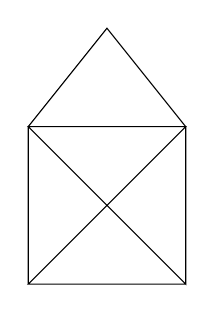
\begin{tikzpicture}
\draw (0,0) -- (0,2) -- (1,3.25) -- (2,2) -- (2,0) -- (0,2) -- (2,2) -- (0,0) -- (2,0);
\end{tikzpicture}
    
	\caption[Mit Tikz programmierte Grafik.]{Mit Tikz programmierte Grafik.}
	\label{fig:tikz_house}
\end{figure}

Ein etwas umfangreicheres Beispiel zur Digitaltechnik ist in Abbildung~\ref{fig:tikz_digital} dargestellt:

\begin{figure}[hbt]
	\centering
	\usetikzlibrary{circuits.logic.US,circuits.logic.IEC}
      \begin{tikzpicture}[circuit logic US]
      \matrix[column sep=7mm]
      {
      \node (i0) {0}; & & \\
      & \node [and gate] (a1) {}; & \\
      \node (i1) {0}; & & \node [or gate] (o) {};\\
      & \node [nand gate] (a2) {}; & \\
      \node (i2) {1}; & & \\
      };
      \draw (i0.east) -- ++(right:3mm) |- (a1.input 1);
      \draw (i1.east) -- ++(right:3mm) |- (a1.input 2);
      \draw (i1.east) -- ++(right:3mm) |- (a2.input 1);
      \draw (i2.east) -- ++(right:3mm) |- (a2.input 2);
      \draw (a1.output) -- ++(right:3mm) |- (o.input 1);
      \draw (a2.output) -- ++(right:3mm) |- (o.input 2);
      \draw (o.output) -- ++(right:3mm) node [right] {$y$ \quad Hier könnte Ihre Formel $y=(0 \land 0) \lor \overline{( 0 \land 1)}$ stehen};
 \end{tikzpicture}

	\caption[Mit Tikz programmierte Grafik, welche bereits vorgefertigte Bibliotheken für Symbole aus der Digitaltechnik nutzt.]{Mit Tikz programmierte Grafik, welche bereits vorgefertigte Bibliotheken für Symbole aus der Digitaltechnik nutzt.}
	\label{fig:tikz_digital}
\end{figure}

\clearpage

In der Tikz-Umgebung können auch Diagramme mit dem \textit{pgfplot}-Befehlssatz erzeugt werden. In Abbildung \ref{fig:pgfplot} sehen Sie ein Beispiel.

\begin{figure}[hbt]
	\centering
	\begin{tikzpicture}
		\begin{axis}[scale=1.3,legend entries={Messwerte mit Fehlerbalken,
			$\pgfmathprintnumber{\pgfplotstableregressiona} \cdot x  
			\pgfmathprintnumber[print sign]{\pgfplotstableregressionb}$}, legend style={draw=none},legend style={at={(0.01,0.98)},anchor=north west},xlabel=Stromstärke $I \; \mathrm{ \lbrack mA \rbrack}$,ylabel=Spannung $U \; \mathrm{ \lbrack V \rbrack}$]
		\addlegendimage{mark=*,blue}
		\addlegendimage{no markers,red}
\addplot+[error bars/.cd, y dir=both,y explicit]
table[x=x,y=y,y error=errory] 
{pgfplot/messdaten_mitfehler.dat};
\addplot table[mark=none,y={create col/linear regression={y=y}}]
{pgfplot/messdaten_mitfehler.dat};
	\end{axis}
\end{tikzpicture}
	\caption[Diagramm, erstellt mit dem \textit{pgfplot}-Befehlssatz.]{Ein Diagramm, erstellt in der \textit{tikzpicture}-Umgebung mit dem \textit{pgfplot}-Befehlssatz. Das Diagramm stellt Messdaten, deren Fehlerbalken und eine Regressionskurve dar. Die Messdaten werden von einer separaten Datei eingelesen und die Regressionskurve wurde mit \textit{pgfplot} berechnet und erstellt.}
	\label{fig:pgfplot}
\end{figure}

\clearpage

Auch hierzu der Quellcode in Listing~\ref{lst:pgfplot}.

\begin{lstlisting}[caption=Quellcode der Abbildung~\ref{fig:pgfplot}.,label=lst:pgfplot]
\begin{figure}[hbt]
\centering
\begin{tikzpicture}
		\begin{axis}[scale=1.3,legend entries={Messwerte mit Fehlerbalken,
			$\pgfmathprintnumber{\pgfplotstableregressiona} \cdot x  
			\pgfmathprintnumber[print sign]{\pgfplotstableregressionb}$}, legend style={draw=none},legend style={at={(0.01,0.98)},anchor=north west},xlabel=Stromstärke $I \; \mathrm{ \lbrack mA \rbrack}$,ylabel=Spannung $U \; \mathrm{ \lbrack V \rbrack}$]
		\addlegendimage{mark=*,blue}
		\addlegendimage{no markers,red}
\addplot+[error bars/.cd, y dir=both,y explicit]
table[x=x,y=y,y error=errory] 
{pgfplot/messdaten_mitfehler.dat};
\addplot table[mark=none,y={create col/linear regression={y=y}}]
{pgfplot/messdaten_mitfehler.dat};
	\end{axis}
\end{tikzpicture}
\caption[Diagramm, erstellt mit dem \textit{pgfplot}-Befehlssatz.]{Ein Diagramm, erstellt in der \textit{tikzpicture}-Umgebung mit dem \textit{pgfplot}-Befehlssatz. Das Diagramm stellt Messdaten, deren Fehlerbalken und eine Regressionskurve dar. Die Messdaten werden von einer separaten Datei eingelesen und die Regressionskurve wurde mit \textit{pgfplot} berechnet und erstellt.}
\label{fig:pgfplot}
\end{figure}
\end{lstlisting}

In Listing~\ref{lst:tikz} ist der Quellcode der Datei \textit{mess\_fehlerbalken.tex} dargestellt.

\begin{lstlisting}[caption=Quellcode der Datei \textit{mess\_fehlerbalken.tex}.,label=lst:tikz]
\begin{tikzpicture}
\begin{axis}[scale=1.3,legend entries={Messwerte mit Fehlerbalken,
$\pgfmathprintnumber{\pgfplotstableregressiona} \cdot x  
\pgfmathprintnumber[print sign]{\pgfplotstableregressionb}$}, legend style={draw=none},legend style={at={(0.01,0.98)},anchor=north west},xlabel=Stromstärke $I \; \mathrm{ \lbrack mA \rbrack}$,ylabel=Spannung $U \; \mathrm{ \lbrack V \rbrack}$]
\addlegendimage{mark=*,blue}
\addlegendimage{no markers,red}
\addplot+[error bars/.cd, y dir=both,y explicit]
table[x=x,y=y,y error=errory] 
{pgfplot/messdaten_mitfehler.dat};
\addplot table[mark=none,y={create col/linear regression={y=y}}]
{pgfplot/messdaten_mitfehler.dat};
\end{axis}
\end{tikzpicture}
\end{lstlisting}

\clearpage

In Abbildung~\ref{fig:pgfplot2y} wird ein weiters Beispiel für ein Diagramm gezeigt. Oftmals wird eine zweite y-Achse verwendet, um verschiedene Skalen darstellen zu können.

\begin{figure}[hbt]
	\centering
	\begin{tikzpicture}
%
\begin{axis}[
scale=1.3,
ytick pos=left,
xlabel=Zeit $t \; \mathrm{ \lbrack ns \rbrack}$,
ylabel=Spannung $U \; \mathrm{ \lbrack V \rbrack}$
]
\addplot[mark=*,only marks] table[x=x,y=y1] {pgfplot/messdaten_zweiyachsen.dat};
\end{axis}
%
\begin{axis}[
scale = 1.3,
legend style={draw=none},
legend style={at={(0.75,0.6)},
anchor=north west},
axis y line*=right,
axis x line=none,
%ymin=0,
%ymax=100,
ylabel=Strom $I \; \mathrm{ \lbrack mA \rbrack}$
]
\addlegendimage{mark=*,only marks}
\addlegendentry{Spannung}
\addplot[mark=x,only marks,blue] table[x=x,y=y2] {pgfplot/messdaten_zweiyachsen.dat};
\addlegendentry{Strom}
\end{axis}
\end{tikzpicture}
	\caption[Diagramm mit zwei unterschiedlichen y-Achsen.]{Diagramm mit zwei unterschiedlichen y-Achsen.}
	\label{fig:pgfplot2y}
\end{figure}

\clearpage

\subsection{Tabellen}

\begin{table}[hbt]	
	\centering
	\renewcommand{\arraystretch}{1.5}	% Skaliert die Zeilenhöhe der Tabelle
	\captionabove[Liste der verwendeten Messgeräte]{Liste der verwendeten Messgeräte. Die Genauigkeitsangaben beziehen sich auf die Standardabweichung $1\cdot \sigma$.}
	\label{tab:bsp}
	\begin{tabular}{ccccc}
		\textbf{Messgerät} & \textbf{Hersteller} & \textbf{Typ} & \textbf{Verwendung} & \textbf{Genauigkeit}\\ 
		\hline 
		\hline 
		\parbox[t]{0.2\linewidth}{\centering Spannungs-\\versorgung} & Voltmaker & HV2000 & \parbox[t]{0.2\linewidth}{\centering Spannungs-\\versorgung der\\Platine} & $\Delta U = \pm 5 $~mV \\ % Der parbox-Befehl ist erforderlich, damit ein Zeilenumbruch erzeugt werden kann. c-Spalten (zentriert) erlauben nicht automatisch einen Zeilenumpruch. Linksbündig gesetzte p-Spalten erlauben automatisch den Zeilenumbruch.
		Strommessgerät & Currentcount & Hotamp 16 & \parbox[t]{0.2\linewidth}{ \centering Strommessung\\am Versorgungspin\\des µC} & $\Delta I = \pm 0.1$~A \\ 
		\hline 
	\end{tabular} 
\end{table}

Der Quellcode der Beispieltabelle~\ref{tab:bsp} ist in Listing~\ref{lst:tab} zu sehen.

\begin{lstlisting}[caption=Quellcode der Tabelle~\ref{tab:bsp}.,label=lst:tab]
\begin{table}[hbt]	
\centering
\renewcommand{\arraystretch}{1.5}	% Skaliert die Zeilenhöhe der Tabelle
\captionabove[Liste der verwendeten Messgeräte]{Liste der verwendeten Messgeräte. Die Genauigkeitsangaben beziehen sich auf die Standardabweichung $1\cdot \sigma$.}
\label{tab:bsp}
\begin{tabular}{ccccc}
\textbf{Messgerät} & \textbf{Hersteller} & \textbf{Typ} & \textbf{Verwendung} & \textbf{Genauigkeit}\\ 
\hline 
\hline 
\parbox[t]{0.2\linewidth}{\centering Spannungs-\\versorgung} & Voltmaker & HV2000 & \parbox[t]{0.2\linewidth}{\centering Spannungs-\\versorgung der\\Platine} & $\Delta U = \pm 5 $~mV \\ % Der parbox-Befehl ist erforderlich, damit ein Zeilenumbruch erzeugt werden kann. c-Spalten (zentriert) erlauben nicht automatisch einen Zeilenumpruch. Linksbündig gesetzte p-Spalten erlauben automatisch den Zeilenumbruch.
Strommessgerät & Currentcount & Hotamp 16 & \parbox[t]{0.2\linewidth}{ \centering Strommessung\\ am Versorgungspin\\ des \textmu C} & $\Delta I = \pm 0.1$~A \\ 
\hline 
\end{tabular} 
\end{table}
\end{lstlisting}

\clearpage

\subsection{Formeln}

Formeln lassen sich in \LaTeX~ganz einfach schreiben. Es gibt unterschiedliche Umgebungen zum Schreiben von Formeln. Z.B. direkt im Text $v=s/t$ oder abgesetzt

\[F=m \cdot a\]

oder auch, wie in wissenschaftlichen Dokumenten üblich, nummeriert

\begin{equation}
P=\frac{U^2}{R} \quad .
\label{eqn:leistung}
\end{equation}

Mit einem Label in Formel~\ref{eqn:leistung} lassen sich natürlich auch Formeln im Text referenzieren. \LaTeX~verwendet im Formelmodus einen eigenen Schriftsatz, welcher entsprechend der gängigen Konventionen kursive Zeichen verwendet. Sollen im Formelmodus Einheiten in normaler Schriftart eingefügt werden, dann kann dies über den Befehl \textbackslash \textit{mathrm}\{\} erwirkt werden, wie im Quellcode von Formel~\ref{eqn:leistungMitEinh} zu sehen ist.

\begin{equation}
P=\frac{U^2}{R} = \frac{\left( 100~\mathrm{V}\right)^2}{100~\Omega} = 100~\mathrm{W}\quad .
\label{eqn:leistungMitEinh}
\end{equation}

Zum direkten Vergleich sind die Einheiten in Formel~\ref{eqn:leistungMitEinhfalsch} falsch dargestellt:

\begin{equation}
P=\frac{U^2}{R} = \frac{\left( 100~V\right)^2}{100\,\varOmega} = 100\,W
\label{eqn:leistungMitEinhfalsch}
\end{equation}

Zur einfachen Eingabe von Einheiten kann auch das Package \textbackslash \textit{siunitx} verwendet werden:

\begin{equation}
	P=\SI{100}{\watt}=\SI{100}{\joule\per\second}
\end{equation}

Das sind nur ein paar wenige Beispiele und es gibt sehr viele Packages, um Besonderheiten in Formeln realisieren zu können, z.B. mehrzeilige Formeln mit vertikaler Ausrichtung. Nennen Sie Formeln nur, wenn diese zum besseren Verständnis auch wirklich nützlich sind.

Folgende Befehle sind innerhalb von Formel-Umgebungen nützlich:
\begin{tabbing}
	\hspace*{0cm} \= \hspace{0.35\linewidth} \= \+\kill
	\textbackslash \textit{text}\{\}	\> Damit kann in Formel-Umgebung Text geschrieben werden.\\ 
	\textbackslash, \textbackslash: \textbackslash; oder \textbackslash quad und \textbackslash qquad \> Zusätzlichen Abstand zwischen Symbolen einfügen.\\
	\textbackslash \textit{notag} \> Nummerierung einer bestimmten Formel ausschalten.
\end{tabbing}

Abschließend nochmals ein kleines Beispiel:

\begin{eqnarray}
\sum\limits_{n=1}^\infty f\left(x_n\right)\cdot \Delta x=  \lim\limits_{\Delta x \rightarrow 0} \frac{f\left(x_0+\Delta x\right)-f\left(x_0\right)}{\Delta x} = \frac{\diff f}{\diff x} = \dot{f}(x)
\end{eqnarray}		% Zeile auskommentieren bei finalem Dokument!

\end{document}
